\documentclass[a4paper,10pt]{article}

% ── Geometry & spacing ───────────────────────────────────────────────────────
\usepackage[a4paper,margin=1.7cm,top=1.5cm,bottom=1.7cm]{geometry}
\usepackage[T1]{fontenc}
\usepackage[utf8]{inputenc}
\usepackage{lmodern}
\usepackage{microtype}

% ── Graphics, layout, color, links ──────────────────────────────────────────
\usepackage{graphicx}
\usepackage{float}
\usepackage{subcaption}
\usepackage{booktabs}
\usepackage{array}
\usepackage{xcolor}
\usepackage{tikz}
\usetikzlibrary{shapes.geometric, arrows.meta, positioning, fit, backgrounds, calc}
\usepackage[colorlinks=true, urlcolor=accent, linkcolor=accent, citecolor=accent]{hyperref}
\usepackage{titlesec}
\usepackage{enumitem}
\usepackage{parskip}
\usepackage{tcolorbox}
\tcbuselibrary{skins, breakable}

% ── Brand palette (matches the dashboard's navy + amber) ────────────────────
\definecolor{accent}{HTML}{1E3A8A}     % navy
\definecolor{accentSoft}{HTML}{E0E7FF} % pale blue
\definecolor{warm}{HTML}{B45309}       % amber
\definecolor{warmSoft}{HTML}{FEF3C7}   % pale amber
\definecolor{ink}{HTML}{0F172A}        % near-black
\definecolor{muted}{HTML}{475569}      % slate
\definecolor{leaf}{HTML}{166534}       % forest green

\AtBeginDocument{\color{ink}}

% ── Typography ─────────────────────────────────────────────────────────────
\titlespacing*{\section}{0pt}{8pt plus 2pt minus 2pt}{2pt}
\titlespacing*{\subsection}{0pt}{5pt plus 2pt minus 2pt}{1pt}
\titleformat{\section}
  {\color{accent}\normalfont\Large\bfseries}
  {\thesection}{0.6em}{}[\vspace{-3pt}\color{accent}\rule{\linewidth}{0.5pt}]
\titleformat{\subsection}{\normalfont\bfseries}{\thesubsection}{0.6em}{}

\setlist{nosep, leftmargin=1.2em, topsep=2pt, partopsep=0pt, itemsep=2pt}

\usepackage[labelfont=bf, font=small, skip=2pt]{caption}

\setlength{\parskip}{3.5pt}

% ── Callout boxes ──────────────────────────────────────────────────────────
\newtcolorbox{decision}{%
  enhanced, breakable,
  colback=accentSoft, colframe=accent,
  boxrule=0.6pt, arc=2pt,
  left=8pt, right=8pt, top=4pt, bottom=4pt,
  coltitle=white, fonttitle=\bfseries,
  attach boxed title to top left={xshift=6pt, yshift=-2pt},
  boxed title style={colback=accent, colframe=accent, arc=1.5pt, boxrule=0pt},
  title=Design decision}

\newtcolorbox{challenge}{%
  enhanced, breakable,
  colback=warmSoft, colframe=warm,
  boxrule=0.6pt, arc=2pt,
  left=8pt, right=8pt, top=4pt, bottom=4pt,
  coltitle=white, fonttitle=\bfseries,
  attach boxed title to top left={xshift=6pt, yshift=-2pt},
  boxed title style={colback=warm, colframe=warm, arc=1.5pt, boxrule=0pt},
  title=Challenge}

\newtcolorbox{finding}{%
  enhanced, breakable,
  colback=leaf!8, colframe=leaf,
  boxrule=0.6pt, arc=2pt,
  left=8pt, right=8pt, top=4pt, bottom=4pt,
  coltitle=white, fonttitle=\bfseries,
  attach boxed title to top left={xshift=6pt, yshift=-2pt},
  boxed title style={colback=leaf, colframe=leaf, arc=1.5pt, boxrule=0pt},
  title=Finding}

% ── Page style ─────────────────────────────────────────────────────────────
\usepackage{fancyhdr}
\pagestyle{fancy}
\fancyhf{}
\renewcommand{\headrulewidth}{0pt}
\fancyfoot[L]{\small\color{muted}Global Trade Explorer \textbullet{} Process Book}
\fancyfoot[R]{\small\color{muted}\thepage}

% ── Document ────────────────────────────────────────────────────────────────
\begin{document}

% ╔════════════════════════ COVER ════════════════════════╗
\thispagestyle{empty}
\begin{center}
  \vspace*{0.3cm}
  {\color{accent}\rule{\linewidth}{1pt}}\\[10pt]
  {\huge\bfseries Global Trade Explorer}\\[4pt]
  {\Large\color{muted}\itshape Dependencies, Flows \& Disruptions}\\[8pt]
  {\large COM-480 Data Visualization \textbullet{} Process Book}\\[4pt]
  {\normalsize Team \textbf{Vizion} \textbullet{} Nicolas Khamis \& Charbel Raffoul \textbullet{} EPFL, Spring 2026}\\[6pt]
  {\color{accent}\rule{\linewidth}{1pt}}
\end{center}

\vspace{0.2cm}

\begin{figure}[H]
  \centering
  \includegraphics[width=\linewidth]{screenshots/00_hero.png}
\end{figure}

\vspace{-6pt}
\begin{center}
\small\color{muted}\itshape
The deployed dashboard: choropleth entry point with year slider, commodity selector,
and click-to-drill country panel. \href{https://vizion-lzz6.onrender.com}{\textbf{vizion-lzz6.onrender.com}}
\end{center}

\vspace{0.2cm}

\begin{tcolorbox}[colback=accentSoft, colframe=accent, boxrule=0.6pt, arc=2pt, left=10pt, right=10pt, top=5pt, bottom=5pt]
\textbf{\color{accent}About this document.}
A reflective process book describing how the Global Trade Explorer was built across
three milestones: from framing trade dependency as a structural question, through
exploratory analysis on UN Comtrade, to a deployed multi-commodity interactive
dashboard. We cover the path we took, the design decisions we made, the challenges
we hit, and how the work was split across the team.
\end{tcolorbox}

\vspace{0.4cm}

% ── Project stats sidebar ──────────────────────────────────────────────────
\begin{center}
\begin{tabular}{c@{\hspace{14pt}}c@{\hspace{14pt}}c@{\hspace{14pt}}c@{\hspace{14pt}}c}
\textbf{\color{accent}5} & \textbf{\color{accent}24} & \textbf{\color{accent}393\,k} & \textbf{\color{accent}\textasciitilde 1\,200} & \textbf{\color{accent}7} \\
\small commodities & \small years (2000--2023) & \small Comtrade rows & \small LOC in \texttt{app.py} & \small interactive views
\end{tabular}
\end{center}

\newpage

% ╔════════════════════════ 1. ORIGIN ════════════════════════╗
\section{Origin: framing the right question}

Global trade is the invisible scaffolding of daily life: the wheat in bread, the
steel in buildings, the gas that heats homes. Yet most existing trade dashboards
stop at \emph{totals}: how much was traded, by whom, in what year. We found that
framing unsatisfying. The front-page trade stories of the 2020s, the 2022
European energy shock, the 2020 semiconductor shortage, the Red Sea disruptions,
are not about totals. They are about \emph{structure}: how concentrated each
country's supply chain is, how exposed it is to a single partner, and what
happens when a corridor breaks.

\textbf{Our goal} became: build an interactive web dashboard that makes the
\emph{structure} of global trade legible, not just its volume. A user picks a
commodity family (energy, cereals, steel, machinery, vehicles), and the
dashboard answers three questions:
\begin{enumerate}
  \item \textbf{Who trades what with whom?} (choropleth, Sankey)
  \item \textbf{How dependent is each country, and on whom?} (top-partner share, top-3 share, HHI)
  \item \textbf{How has this structure shifted, and what would happen if it were disrupted?} (top movers, dependency race, planned disruption simulator)
\end{enumerate}

Existing platforms (OEC, World Bank, UN Comtrade dashboards) answer (1) well and
(2) only partially; none address (3) interactively. That gap defined the project.

\subsection{Audience and design principle}

The target audience is students, researchers, journalists, and engaged
citizens with an interest in global economics or supply-chain resilience.
They are not necessarily economists. From this we extracted the central
design principle drawn from the \emph{Interaction} lecture:

\begin{decision}
\textbf{Progressive disclosure.}
A first-time visitor must understand the dashboard in 10 seconds. A power user
must be able to drill into HHI values, animate dependency over decades, and
compare two countries side-by-side. We keep the front page deliberately simple
(one map, one slider, one commodity dropdown) and push all advanced views into
a tabbed side panel that opens only when a country is clicked.
\end{decision}

% ╔════════════════════════ 2. DATA ════════════════════════╗
\section{The data: UN Comtrade}

We use the \textbf{UN Comtrade database}, which publishes annual bilateral trade
flows at the HS (Harmonized System) product level. Our window is 2000--2023 and
our scope is five HS chapters chosen for their geopolitical salience:
\textbf{HS 27} mineral fuels, \textbf{HS 10} cereals, \textbf{HS 72} iron \&
steel, \textbf{HS 84} machinery, \textbf{HS 87} vehicles. Energy (HS 27) was
the natural pilot; the other four were added once the pipeline generalized.

\begin{figure}[H]
  \centering
  \begin{subfigure}[t]{0.49\linewidth}
    \includegraphics[width=\linewidth]{screenshots/eda_evolution.png}
    \caption{\textbf{Global energy trade, 2000--2023.} The series grows roughly
    6$\times$ over the window (from \$0.7\,T to \$4.0\,T) and four shocks are
    visible: the 2008 financial crisis ($-35$\%), the 2014--16 oil crash, the
    2020 COVID dip ($-25$\%), and the 2022 geopolitical spike. These shocks
    directly informed the dashed annotations in the Trade History tab.}
  \end{subfigure}\hfill
  \begin{subfigure}[t]{0.49\linewidth}
    \includegraphics[width=\linewidth]{screenshots/eda_concentration.png}
    \caption{\textbf{Trade concentration analysis.} A long tail of small
    economies sources $>50$\% of their energy imports from a single partner.
    This skewed distribution motivated the \emph{Dependency} panel's
    diversified / moderate / concentrated bands at 33\% and 50\% (visible in
    panel D on page 4).}
  \end{subfigure}
\end{figure}

The EDA notebook (\texttt{notebooks/01\_exploratory\_data\_analysis.ipynb})
confirmed three things that shaped every downstream choice: \textbf{(a)} trade
values span five orders of magnitude in USD (forcing a log scale on the map);
\textbf{(b)} dependency is heavily skewed; \textbf{(c)} four temporal shocks
structure the entire 24-year window, turning ``show change over time'' into a
richer story than expected.

\subsection{Findings: what the data revealed}

Before building any viz, the EDA already surfaced concrete claims:

\begin{finding}
\textbf{Energy trade more than sextupled between 2000 and 2022}, from
\$0.7\,T to \$4.0\,T, with four discrete shocks (2008, 2014--16, 2020, 2022)
visible in both imports and exports.
\end{finding}
\begin{finding}
\textbf{The top energy importers are the world's largest economies}: USA,
China, Japan, Germany, South Korea, India. The top exporters are a different
set: Russia, Saudi Arabia, Canada, Norway, UAE. Trade is structurally a
producer-vs-consumer split.
\end{finding}
\begin{finding}
\textbf{Smaller economies are the most dependent.} The ``most-import-dependent''
ranking is dominated by Bhutan, State of Palestine, Lesotho, Belarus, and
Liberia, all sourcing $\geq 80$\% of their energy from a single partner. Large
economies (USA, Germany) are well-diversified.
\end{finding}
\begin{finding}
\textbf{Three corridors dominate the energy world.} Canada$\rightarrow$USA is
the single largest globally; Russia$\rightarrow$EU was the second-largest until
2022; the Persian Gulf$\rightarrow$East Asia spine connects the Middle East to
Japan, South Korea, and China.
\end{finding}
\begin{finding}
\textbf{Three countries play both sides.} The USA, the Netherlands, and Belgium
appear simultaneously in the top-importer and top-exporter rankings. The USA
is a genuine dual-role actor; the Netherlands and Belgium are largely re-export
hubs (Rotterdam, Antwerp), which is why we flag re-export inflation as a known
caveat and use direct importer-reported shares for dependency calculations.
\end{finding}
\begin{finding}
\textbf{Shocks are visible in both sides of the ledger.}
Imports and exports tracked each other within 0.2 percentage points
(50.1\% / 49.9\% global balance), which gave us confidence in the data: the
2008 crash, the 2014--16 oil collapse, the 2020 COVID dip, and the 2022 spike
all appear symmetrically in both series.
\end{finding}
\begin{finding}
\textbf{Coverage is uneven across decades.}
The first half of the window (2000--2005) has roughly 30\% fewer reporting
countries than the second half. We kept the slider at 2000--2023 (the early
years are useful as a baseline) but document the caveat and steer
storytelling toward the post-2008 era where coverage is dense.
\end{finding}

\newpage

% ╔════════════════════════ 3. EVOLUTION ════════════════════════╗
\section{From sketch to prototype to product}

\subsection{Milestone 1: framing and EDA}

Milestone 1 was about understanding what we had. We acquired the Comtrade data
via API, built a preprocessing pipeline (\texttt{src/preprocess.py},
\texttt{src/data\_loader.py}, \texttt{src/utils.py}), and produced an
exploratory notebook documenting coverage, shocks, and dependency structure.
The deliverable was a static choropleth and a narrative explaining \emph{why}
the project was worth doing.

\subsection{Milestone 2: the interactive prototype}

We chose \textbf{Dash (Plotly under the hood)} as the framework. The course
nominally asks for D3, but Dash gave us the same interactivity on top of
Plotly's mature geographic and Sankey primitives, in Python rather than a
JavaScript bridge. The course rubric explicitly allows ``D3.js (and other)''.

\begin{decision}
\textbf{Dash + Plotly over raw D3.}
Trade-off: less hand-control over the SVG, but instant access to Plotly's
choropleth, Sankey, and animation frames; the same pandas code that did the
EDA could power the dashboard. The cost was discovering Plotly's quirks
(d3-format's ``G'' suffix, default tick rendering, layout margins) and
working around them; the saving was a week of D3 boilerplate we did not
have to write.
\end{decision}

\subsection{From plan to prototype: M1 findings become M3 views}

Our milestone 1 deliverable consisted of the static EDA figures shown on
page 2 plus a written narrative arguing that \emph{structure}, not totals,
was the interesting question. Those figures \emph{were} the plan: each
static observation set the agenda for a corresponding interactive view in
the dashboard. The mapping below traces that expansion.

\begin{table}[H]
\centering\small
\renewcommand{\arraystretch}{1.25}
\begin{tabular}{@{}p{5.2cm}p{1cm}p{9.6cm}@{}}
\toprule
\textbf{M1 plan (static EDA finding)} & & \textbf{M3 expansion (interactive view)} \\
\midrule
Global energy trade 6$\times$ growth with four shocks visible (line chart, fig.~2a) &
$\rightarrow$ &
\textbf{Trade History tab (B)} with shock-band annotations and click-to-update country selection. \\
Top-1 partner share is heavily skewed (histogram, fig.~2b) &
$\rightarrow$ &
\textbf{Dependency panel (D)} with diversified / moderate / concentrated bands and dual top-1 / top-3 lines over time. \\
Ranking of the most-import-dependent countries (static bar, fig.~2b) &
$\rightarrow$ &
\textbf{Dependency Race (F)} animated ranking across all 24 years and 5 commodities. \\
EDA observation: ``trade is structurally a producer-vs-consumer split'' &
$\rightarrow$ &
\textbf{Compare tab (G)} enabling direct head-to-head comparison of two countries' totals, history, and dependency. \\
EDA observation: three corridors dominate the energy world &
$\rightarrow$ &
\textbf{Sankey flow (C)} showing every country's bilateral structure on demand. \\
Visible YoY shocks (2008, 2020, 2022) in the global series &
$\rightarrow$ &
\textbf{Top Movers (E)} surfacing the biggest movers in every year, every commodity. \\
\bottomrule
\end{tabular}
\end{table}

The pattern is consistent: \emph{static EDA finding $\rightarrow$ interactive
view that lets the user verify it for any country, year, and commodity}. We
did not produce hand-drawn sketches at M1; the EDA figures themselves
\emph{were} the visual plan, and the dashboard is their direct expansion.

\subsection{The seven visualizations}

\begin{figure}[H]
  \centering
  \begin{subfigure}[t]{0.49\linewidth}
    \includegraphics[width=\linewidth]{screenshots/02_history.png}
    \caption{\textbf{(B) Trade History.}
    \emph{Question: how has this country's trade changed?}
    Dual line chart (imports and exports) with the active year highlighted.
    The shock-band annotations let users instantly contextualize a dip:
    is this 2008, 2020, 2022, or something country-specific?
    \emph{Lecture connection:} Time-series \& Annotation.}
  \end{subfigure}\hfill
  \begin{subfigure}[t]{0.49\linewidth}
    \includegraphics[width=\linewidth]{screenshots/03_sankey.png}
    \caption{\textbf{(C) Trade Flows (Sankey).}
    \emph{Question: who does this country buy from and sell to, and in what
    proportion?}
    Ribbon width $\propto$ USD; left = import sources, right = export
    destinations. The orange/blue split mirrors the import/export colour code
    used throughout.
    \emph{Lecture connection:} Graphs \& networks.}
  \end{subfigure}
\end{figure}

\vspace{-8pt}

\begin{figure}[H]
  \centering
  \begin{subfigure}[t]{0.49\linewidth}
    \includegraphics[width=\linewidth]{screenshots/03_dependency.png}
    \caption{\textbf{(D) Dependency.}
    \emph{Question: how concentrated is this country's supply?}
    Top-partner and top-3 partner shares plotted across 2000--2023 with
    diversified / moderate / concentrated bands so a non-expert can read
    risk at a glance.
    \emph{Lecture connection:} Rankings; Perception (banded ranges).}
  \end{subfigure}\hfill
  \begin{subfigure}[t]{0.49\linewidth}
    \includegraphics[width=\linewidth]{screenshots/06_compare.png}
    \caption{\textbf{(G) Compare.}
    \emph{Question: how does country X differ from country Y?}
    Two countries side-by-side on totals, overlaid history, and overlaid
    dependency. Used to contrast peers (Germany vs Japan on steel, USA vs
    China on machinery).
    \emph{Lecture connection:} Small multiples.}
  \end{subfigure}
\end{figure}

\vspace{-8pt}

\begin{figure}[H]
  \centering
  \begin{subfigure}[t]{0.49\linewidth}
    \includegraphics[width=\linewidth]{screenshots/04_movers.png}
    \caption{\textbf{(E) Top Movers.}
    \emph{Question: who shifted the most this year vs last?}
    Diverging bars (green gainers / red losers) of YoY \% change with a
    trade-volume floor so small economies don't dominate the ranking.
    \emph{Lecture connection:} Change over time.}
  \end{subfigure}\hfill
  \begin{subfigure}[t]{0.49\linewidth}
    \includegraphics[width=\linewidth]{screenshots/05_race.png}
    \caption{\textbf{(F) Dependency Race.}
    \emph{Question: which countries are diversifying, which are locking in?}
    Animated ranking of ``\% of imports from top single partner'' across
    24 years, playing back decades of structural change in seconds.
    \emph{Lecture connection:} Animation.}
  \end{subfigure}
\end{figure}

\subsection{Iteration: before \& after}

A handful of fixes that look small in isolation but materially raised the
prototype's readability. We treat these as a record of the craft involved.

\begin{tcolorbox}[colback=warmSoft!50, colframe=warm, boxrule=0.4pt, arc=2pt, left=8pt, right=8pt, top=3pt, bottom=3pt]
\small
\textbf{(i) Currency rendering: \texttt{\$100G} $\rightarrow$ \texttt{\$100B}.}
Plotly's d3-format uses SI prefixes, so \texttt{tickformat="\$.2s"} produced
\texttt{\$100G} (giga) instead of the familiar \texttt{B} (billion). We
dropped the d3 format and used \texttt{tickprefix="\$"} so Plotly's native
formatter (which uses \texttt{B}) takes over, and replaced hover
\texttt{\%\{y:\$.3s\}} with pre-formatted \texttt{customdata} strings.
\\[3pt]
\textbf{(ii) Top Movers \% precision: ``+37.45\%'' $\rightarrow$ ``+37\%''.}
The default printed full float precision in hovers. We changed the format
spec to \texttt{:+.0f} so the chart reads as a structural change, not a
spurious-precision one.
\\[3pt]
\textbf{(iii) RadioItems readability.}
The flow-toggle's default browser-blue radio dots and link-blue label text
were invisible on the dark panel. We set \texttt{labelStyle.color} to the
panel's \texttt{TEXT\_MAIN} and \texttt{inputStyle.accentColor} to the
gainer-green used elsewhere.
\\[3pt]
\textbf{(iv) Compare-tab title \& legend overlap.}
Plotly's default put the title and the legend in the same vertical band.
We widened the top margin to 70\,px and pinned title \texttt{y=0.97},
legend \texttt{y=1.08}, so neither encroached on the other.
\end{tcolorbox}

\subsection{Colour, typography, accessibility}

The interface uses a \textbf{dark base} (\#0F172A / \#1E293B) for the panels
to keep the choropleth's saturated YlOrRd the dominant element. We deliberately
chose a \emph{single-hue sequential} scale rather than a divergent one because
the trade value has no meaningful zero-crossing (the Perception lecture's
discussion of pre-attentive features informed this). Import-orange
(\#F59E0B) and export-blue (\#3B82F6) are used consistently across every
view so a colour acts as a stable signifier. The font stack is the system
sans (San Francisco / Segoe UI / Roboto) for fast rendering and good cross-OS
fidelity. We checked the YlOrRd scale against a deuteranopia simulator and
the ordering remains preserved.

\newpage

% ╔════════════════════════ 4. ARCHITECTURE ════════════════════════╗
\section{Architecture and implementation}

\subsection{Data flow}

\begin{figure}[H]
\centering
\begin{tikzpicture}[
  font=\small,
  node distance=8mm and 10mm,
  box/.style={draw=accent, fill=accentSoft, rounded corners=2pt, minimum height=9mm, minimum width=24mm, align=center, inner sep=3pt},
  src/.style={draw=warm, fill=warmSoft, rounded corners=2pt, minimum height=9mm, minimum width=24mm, align=center, inner sep=3pt},
  out/.style={draw=leaf, fill=leaf!10, rounded corners=2pt, minimum height=9mm, minimum width=24mm, align=center, inner sep=3pt},
  arr/.style={-Latex, accent, thick},
]
  \node[src] (api) {UN Comtrade\\API};
  \node[box, right=of api] (raw) {\texttt{data/raw/}\\\scriptsize HS 10/27/72/84/87\\\scriptsize per-commodity CSVs};
  \node[box, right=of raw] (pp) {\texttt{src/preprocess\_}\\\texttt{multi.py}\\\scriptsize ISO-3 + clean};
  \node[box, right=of pp] (proc) {\texttt{data/processed/}\\\scriptsize country\_summary\\\scriptsize partner\_flow};
  \node[box, below=10mm of proc] (app) {\texttt{app.py} (Dash)\\\scriptsize callbacks + Plotly};
  \node[out, left=of app] (gun) {gunicorn\\\scriptsize 1 worker, 120s};
  \node[out, left=of gun] (web) {Render free tier\\\scriptsize eu-frankfurt};
  \node[out, left=of web] (user) {Browser};

  \draw[arr] (api) -- (raw);
  \draw[arr] (raw) -- (pp);
  \draw[arr] (pp) -- (proc);
  \draw[arr] (proc) -- (app);
  \draw[arr] (app) -- (gun);
  \draw[arr] (gun) -- (web);
  \draw[arr] (web) -- (user);
\end{tikzpicture}
\caption*{\small From a single API call to a pixel on the user's screen. Build-time
artefacts (orange) are produced once; runtime artefacts (green) are spun up by
Render on each cold start.}
\end{figure}

\vspace{-6pt}

\subsection{Layered stack}

\begin{table}[H]
\centering\small
\begin{tabular}{@{}p{4.0cm}p{11.7cm}@{}}
\toprule
\textbf{Layer} & \textbf{What we used} \\
\midrule
Data ingestion & UN Comtrade API via \texttt{comtradeapicall};
\texttt{src/download\_comtrade.py} (HS 27) and
\texttt{src/download\_multi\_commodity.py} (HS 10, 72, 84, 87) \\
Preprocessing & pandas, NumPy; \texttt{src/preprocess.py},
\texttt{src/preprocess\_multi.py}; ISO-3 normalization in \texttt{src/utils.py} \\
Exploratory analysis & Jupyter notebooks in \texttt{notebooks/}; matplotlib for
static figures saved to \texttt{outputs/figures/} \\
Frontend \& interactivity & Dash 2.x (Plotly under the hood); a single
\texttt{app.py} with Dash callbacks; no separate JS toolchain \\
Visualizations & Plotly \texttt{choropleth}, \texttt{scatter} (history),
\texttt{sankey} (flows), \texttt{bar} (dependency / movers / race),
\texttt{frames} (race animation) \\
Hosting & Render free tier (\textsc{eu-frankfurt}), gunicorn with
\texttt{server = app.server}; \texttt{render.yaml} pins Python 3.11; auto-deploy
on \texttt{git push origin main} \\
Source control & Two-remote workflow: personal
\texttt{NicolasKhms/global\_trade\_viz} as a safety net, class
\texttt{com-480-data-visualization/Vizion} as the submission target \\
\bottomrule
\end{tabular}
\end{table}

\subsection{From a fresh clone to a running app}

\begin{tcolorbox}[colback=warmSoft!50, colframe=warm, boxrule=0.4pt, arc=2pt, fontupper=\ttfamily\small, left=8pt, right=8pt]
git clone https://github.com/com-480-data-visualization/Vizion\\
cd Vizion \&\& python3 -m venv .venv \&\& source .venv/bin/activate\\
pip install -r requirements.txt\\
python app.py\hspace{2em}\# http://127.0.0.1:8050
\end{tcolorbox}

For the public demo no setup is needed:
\href{https://vizion-lzz6.onrender.com}{vizion-lzz6.onrender.com}
(first request after inactivity cold-starts for $\sim$30--60\,s).

% ╔════════════════════════ 5. CHALLENGES ════════════════════════╗
\section{Challenges and design decisions}

\subsection{Data engineering}

\begin{challenge}
\textbf{The UN Comtrade free tier limits us to 500 API calls per day.}
The world has 200+ reporting countries and we need 24 years across 5
commodities, well beyond a single day's quota.
\end{challenge}
\begin{decision}
\textbf{Aggressive caching per commodity.}
We download once per HS chapter into a single raw CSV, then build derived files
that the app loads at startup. Re-running the dashboard never re-hits the API.
\end{decision}

\begin{challenge}
\textbf{About 10\% of partner rows have no ISO-3 code} (inconsistent spellings,
aggregate entities like ``World'' and ``Areas, nes'').
\end{challenge}
\begin{decision}
\textbf{Manual override table + hard exclusion list} in \texttt{src/utils.py};
aggregates are filtered out before any bilateral analysis, so the choropleth
never tries to colour ``World''.
\end{decision}

\begin{challenge}
\textbf{Re-export inflation for hub countries (NLD, BEL, SGP)} makes naive
top-partner counts misleading: these countries re-route huge volumes they
neither consume nor produce.
\end{challenge}
\begin{decision}
\textbf{Direct importer-reported share as the headline metric}, caveat
documented in the EDA. We chose not to attempt re-export attribution (its
own research problem) but the metric we display answers the user's actual
resilience question.
\end{decision}

\subsection{Visualization \& UX}

\begin{challenge}
\textbf{Trade values span five orders of magnitude.}
On a linear colour scale, everyone outside the top 10 looked identical.
\end{challenge}
\begin{decision}
\textbf{Log-scaled choropleth.}
Surfaces small-but-significant traders (Switzerland, Austria) without
losing the giants. We confirmed against
\texttt{outputs/figures/00\_trade\_value\_distribution.png} before committing.
\end{decision}

\begin{challenge}
\textbf{Information overload.}
Showing flows + history + dependency + compare at once overwhelms the user,
but hiding them defeats the purpose.
\end{challenge}
\begin{decision}
\textbf{Tabs inside the country side panel.}
The main view stays clean (just the map); a click opens a side panel with four
tabs. Practical embodiment of the progressive-disclosure principle.
\end{decision}

\subsection{Engineering \& deployment}

\begin{challenge}
\textbf{Render's free tier caps memory at 512\,MB.}
All five commodity datasets in pandas use 300--500\,MB at peak, right on
the edge of the cap.
\end{challenge}
\begin{decision}
\textbf{Single-worker gunicorn + 120\,s startup timeout.}
\texttt{--workers 1} keeps a single in-memory copy; \texttt{--timeout 120}
covers the cold-start CSV load. Lazy-loading was the planned fallback but the
dashboard fit without it.
\end{decision}

\begin{challenge}
\textbf{Raw energy file is 122\,MB, above GitHub's 100\,MB per-file limit.}
We need data committed so a fresh container can boot, but GitHub rejects it.
\end{challenge}
\begin{decision}
\textbf{Whitelist-based \texttt{.gitignore}.}
Ignore everything in \texttt{data/processed/} by default, then explicitly
re-include the small derived files the app loads
(\texttt{*\_country\_summary.csv}, \texttt{*\_partner\_flow.csv}). The 122\,MB
raw aggregate stays out; the deploy still works.
\end{decision}

\newpage

% ╔════════════════════════ 6. CASE STUDY ════════════════════════╗
\section{Case study: the Dependency panel}

The Dependency panel (view D) is the most distinctive part of the dashboard
and the one that took the longest to settle on. This is its design history.

\textbf{The question.} \emph{For a given country and commodity, how
concentrated is the import side over time, and is it improving or
worsening?} An economist would answer with the Herfindahl-Hirschman Index;
a journalist would say ``what \% comes from one partner?''. We need both
to land at once.

\textbf{Alternatives we considered.}
\begin{itemize}
  \item \emph{Stacked bar of top-5 partners, year on x-axis.}
  Rejected: the eye can't compare partner shares across years easily
  because every band shifts position.
  \item \emph{Pie chart of partner shares for a single year.}
  Rejected: discards the temporal dimension, which is half the story.
  \item \emph{HHI line alone.}
  Rejected: the HHI is opaque to a non-economist; it scores ``low'' at
  0.15 but most readers would not know whether that is good or bad.
  \item \emph{A pair of lines: top-1 share and top-3 share, with
  contextual bands.} \textbf{Chosen.} Two intuitive numbers, both moving
  through time, with banded background colour
  (\emph{diversified / moderate / concentrated}) so a reader without an
  economics background can read risk at a glance.
\end{itemize}

\begin{decision}
\textbf{Two metrics, not one; bands, not labels.}
A single dependency score (HHI) is precise but unreadable. Two
intuitive metrics (top-1 and top-3 share) plus three labelled regions
let the user understand structure \emph{and} risk in one view, without
prior economics training.
\end{decision}

\textbf{What the user can extract.} A glance at Switzerland (panel D on
page 4) tells the story: top-1 share rose from $\sim$20\% in 2000 to a
moderate $\sim$40\% by 2010 and has stabilised since; top-3 share has
sat above 60\% for two decades, putting Switzerland firmly in the
moderately-concentrated band. Compare Germany 2018 (well-diversified)
to Germany 2023 (climbing toward concentrated after the Russia pivot)
and the panel does the talking.

% ╔════════════════════════ 7. REFLECTION ════════════════════════╗
\section{Reflection}

\subsection{What we would do differently}

\textbf{Start with the dependency story sooner.} We spent the first weeks
on choropleth polish; the dependency view (now the dashboard's most
distinctive feature) only landed in the second prototype iteration. In
hindsight, the structural questions \emph{were} the project from day
one; the choropleth is just the entry point.

\textbf{Budget more time for performance.} Render's cold start is fine
for graders but mediocre for real users. A future iteration would
pre-aggregate per-country JSON blobs at preprocessing time and serve
them as static files, eliminating the pandas-in-memory dependency.

\textbf{Build the disruption simulator early.} It is the headline
differentiator versus OEC and World Bank dashboards; pushing it to M3
meant we could not iterate on it.

\subsection{Known limitations}

\begin{itemize}
  \item Values are in nominal USD; no inflation adjustment is applied,
  so absolute magnitudes inflate over time.
  \item Mirror-trade asymmetry is not reconciled; we prefer
  importer-reported values for dependency calculations.
  \item Re-export inflation is documented but not corrected.
  \item 2023 coverage is incomplete (some reporters had not filed yet
  when we pulled the data).
  \item Cold start on Render's free tier is 30--60\,s.
\end{itemize}

% ╔════════════════════════ 8. PEER ════════════════════════╗
\section{Peer assessment}

The split below is based on the git history on the class repository,
cross-checked against the team's working notes.

\begin{table}[H]
\centering\small
\begin{tabular}{@{}p{4.3cm}p{8cm}p{3cm}@{}}
\toprule
\textbf{Area} & \textbf{Tasks} & \textbf{Owner} \\
\midrule
Project scaffold & Initial repo, Milestone 1 PDF, README folder structure & Charbel Raffoul \\
Data acquisition & Comtrade API integration, HS 27 pipeline & Nicolas Khamis \\
EDA \& notebooks & Quality assessment, exploratory analysis, shock ID & Nicolas Khamis \\
Multi-commodity pipeline & HS 10/72/84/87 downloads, schema unification & Nicolas Khamis \\
Dashboard core & Choropleth, slider, country side panel & Nicolas Khamis \\
Tabbed views & Trade History, Sankey, Dependency, Compare & Nicolas Khamis \\
Global rows & Top Movers, Dependency Race & Nicolas Khamis \\
Visual polish & Palette, currency formatting, layout tuning & Nicolas Khamis \\
Deployment & Render config, gunicorn, \texttt{.gitignore} whitelist & Nicolas Khamis \\
Reports \& process book & M1 notes, M2 report, this process book & Nicolas \& Charbel \\
Screencast & Script, recording, editing & {\color{muted}\itshape (M3, TBD)} \\
\bottomrule
\end{tabular}
\end{table}

\subsection{Project timeline}

\begin{figure}[H]
\centering
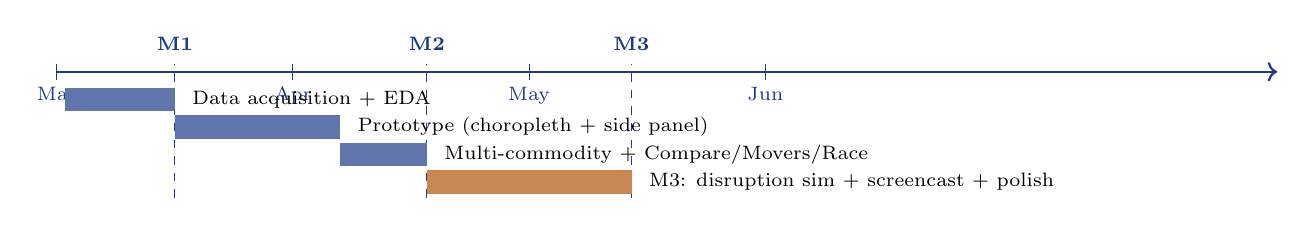
\begin{tikzpicture}[font=\scriptsize]
  % Time axis
  \draw[->, thick, accent] (0,0) -- (15.5,0);
  \foreach \x/\m in {0/Mar, 3/Apr, 6/May, 9/Jun} {
    \draw[accent] (\x,-0.1) -- (\x,0.1);
    \node[below=2pt, accent] at (\x,0) {\m};
  }
  % Milestones
  \node[above, accent, font=\scriptsize\bfseries] at (1.5,0.15) {M1};
  \node[above, accent, font=\scriptsize\bfseries] at (4.7,0.15) {M2};
  \node[above, accent, font=\scriptsize\bfseries] at (7.3,0.15) {M3};
  \draw[dashed, accent] (1.5,-1.6) -- (1.5,0.1);
  \draw[dashed, accent] (4.7,-1.6) -- (4.7,0.1);
  \draw[dashed, accent] (7.3,-1.6) -- (7.3,0.1);
  % Tasks
  \fill[accent!70] (0.1,-0.5) rectangle (1.5,-0.2);
  \node[right] at (1.6,-0.35) {\scriptsize Data acquisition + EDA};
  \fill[accent!70] (1.5,-0.85) rectangle (3.6,-0.55);
  \node[right] at (3.7,-0.7) {\scriptsize Prototype (choropleth + side panel)};
  \fill[accent!70] (3.6,-1.2) rectangle (4.7,-0.9);
  \node[right] at (4.8,-1.05) {\scriptsize Multi-commodity + Compare/Movers/Race};
  \fill[warm!70] (4.7,-1.55) rectangle (7.3,-1.25);
  \node[right] at (7.4,-1.4) {\scriptsize M3: disruption sim + screencast + polish};
\end{tikzpicture}
\end{figure}

\begin{center}
\small\color{muted}\itshape
\rule{0.4\linewidth}{0.4pt}\\[4pt]
Thank you for reading.
Live dashboard: \href{https://vizion-lzz6.onrender.com}{vizion-lzz6.onrender.com}.
Code: \href{https://github.com/com-480-data-visualization/Vizion}{github.com/com-480-data-visualization/Vizion}.
\end{center}

\end{document}
